LeNetはDeep Learningの根幹ともいえるCNNアーキテクチャで,図\ref{arch_lenet}に示す構造を持つ \cite{arxiv_lenet} \cite{arch_lenet}.誤差逆伝播法による学習で,MNIST\footnote{THE MNIST DATABASE of handwritten digits, \url{http://yann.lecun.com/exdb/mnist/}}などの文字認識で高精度を実現した.

\begin{figure} [H]
	\begin{center}
		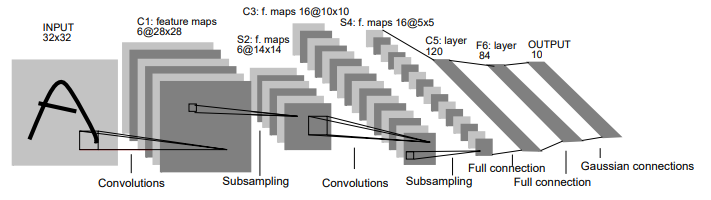
\includegraphics[clip, height=5cm, bb=-30 0 711 200]{data/figure/arch_lenet.png}
		\caption{LeNetアーキテクチャ}
		\label{arch_lenet}
	\end{center}
\end{figure}
